\section{Codestatistik}
	Für \eeppi\ haben wir drei verschiedene Arten von Codestatistiken.
	Die erste Statistik zeigt den Umfang des Projekts,
	die zweite wie gut wir getestet haben
	und die dritte wie "'schön"' der Code ist.
	Der Client wurde mit TypeScript entwickelt und dieses wurde dann zu JavaScript kompiliert.
	Die Codestatistik über den Umfang wurde für den Clientteil mit den TypeScript-Dateien durchgeführt,
	die restlichen Statistiken danach mit den JavaScript-Dateien.
	
	\subsection{Umfang}
	Total hat \eeppi\ gut 25'000 Zeilen Code, dabei ist alles gezählt,
	also auch Leerzeilen, Kommentare, Konfigurationsdaten und gar Code von anderen Entwicklern.
	Die Aufteilung in die verschiedenen Kategorien ist in Abbildung\ \ref{fig:TotalSLOC} zu sehen.
	\begin{figure}[H]
		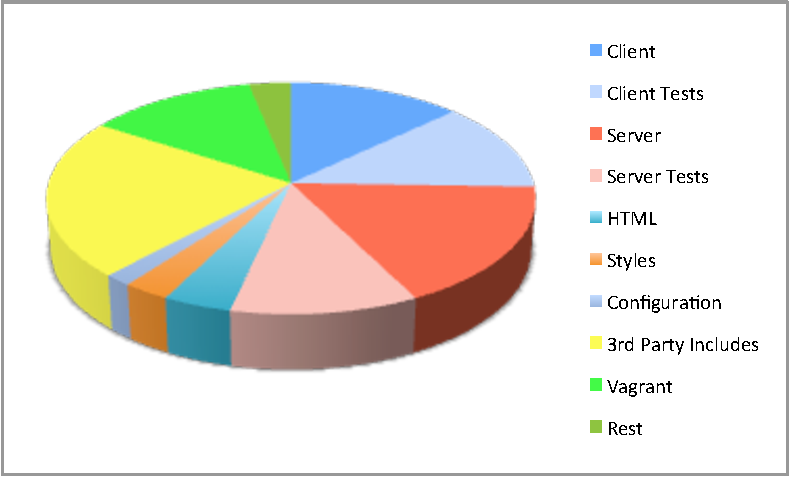
\includegraphics[width=\largeThird\textwidth]{projectPlan/media/img/totalSLOC.pdf}
		\centering
		\caption{Total SLOC (Source Lines of Code)}
		\label{fig:TotalSLOC}
	\end{figure}
	
	Gut die Hälfte des Umfangs machen dabei die rechnenden Teile des Servers und des Clients aus,
	zusammen mit den Tests.
	Ein weiterer grosser Brocken sind die externen Abhängigkeiten (22\%),
	sowie die Daten für die Initialkonfiguration der Vagrant-Umgebungen.
	Der ganze Rest des Projekts macht noch 12\% aus,
	dazu gehören die Daten nötig für die Anzeige sowie die Konfigurationsdaten.
	
	Wenn man den Hauptteil von \eeppi, also die (rechnenden) Server- und Client-Teile genauer anschaut,
	so sieht man, dass die Server- und die Client-Teile eine Grösse in der gleichen Dimension haben.
	Dies ist auch so zu erwarten, da sie auch den gleichen Umfang der Daten verarbeiten.
	
	Und auch die Tests sind in der gleichen Grössenordnung.
	Die Client-Tests haben jedoch hier im Vergleich einen überproportionalen Anteil,
	dies ist auf "'zeilenhungrige"' Initialisierungsdaten darin zurückzuführen.
	Die genaue Aufteilung und die genaue Anzahl der SLOC (Source Lines of Code) des Hauptteils ist in Abbildung\ \ref{fig:serverClientSLOC} zu sehen.
	\begin{figure}[H]
		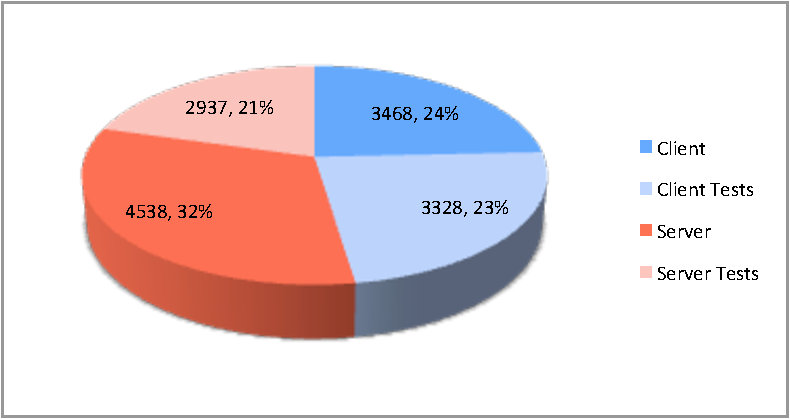
\includegraphics[width=\largeThird\textwidth]{projectPlan/media/img/serverClientSLOC.pdf}
		\centering
		\caption{Vergleich SLOC (Source Lines of Code) auf Server und Client mit den Tests}
		\label{fig:serverClientSLOC}
	\end{figure}

	\subsection{Test Coverage}
	Sowohl auf dem Server als auch auf dem Client haben wir mehrheitlich mit der Methode des TDD (Test Driven Developments) entwickelt,
	dementsprechend haben wir auch eine gute Testabdeckung.
	Das Ziel war nicht 100\% Testabdeckung zu erreichen, sondern die wichtigsten Funktionen zu testen.
	\begin{figure}[H]
		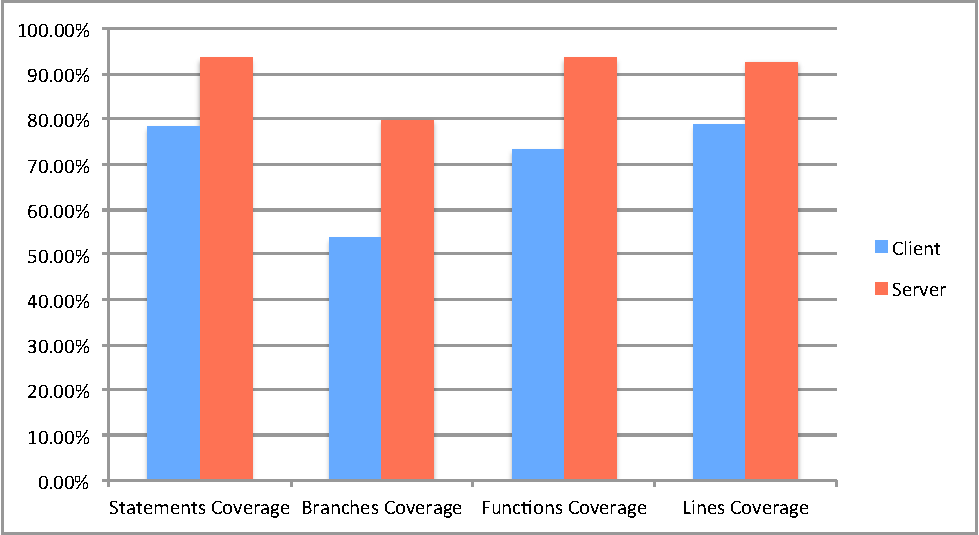
\includegraphics[width=\textwidth]{projectPlan/media/img/coverage.pdf}
		\centering
		\caption{Testabdeckung auf dem Server und dem Client}
		\label{fig:coverage}
	\end{figure}
	In Abbildung\ \ref{fig:coverage} ist die Testabdeckung aufgezeigt.
	Es ist zu sehen, dass auf dem Server die Testabdeckung höher ist als auf dem Client,
	aber auch auf dem Client sind die zentralen und wichtigen Elemente gut getestet.
	
	\subsection{Qualität}
	Die Codequalität wirklich zu messen ist quasi ein Ding der Unmöglichkeit.
	Für \eeppi\ haben wir jedoch einige Kennzahlen evaluiert,
	nämlich die Anzahl der Logical LOC, die Anzahl der Parameter und die Cyclomatic Complexity.
	\begin{figure}[H]
		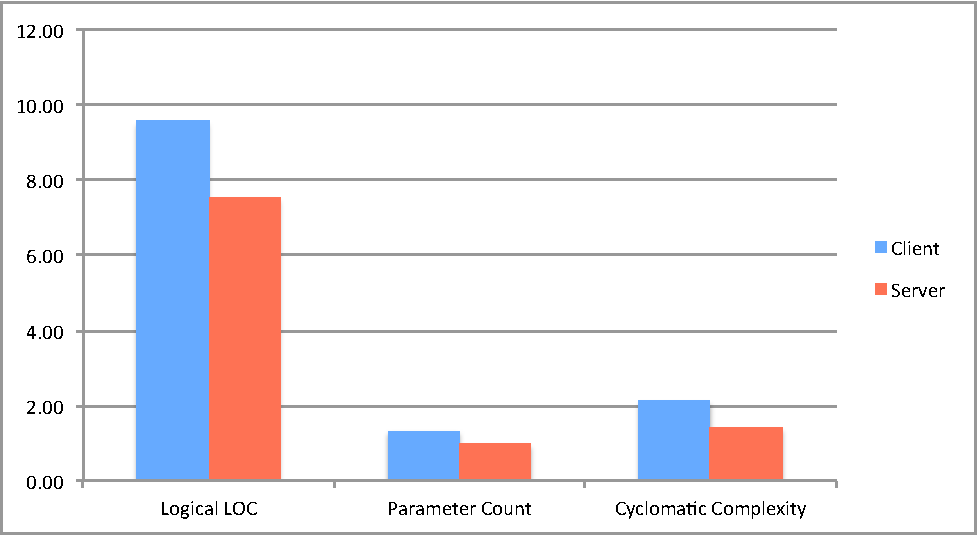
\includegraphics[width=\textwidth]{projectPlan/media/img/methodComplexityOverview.pdf}
		\centering
		\caption{Überblick Komplexitätskennwerte pro Methode (Durchschnitt)}
		\label{fig:methodComplexityOverview}
	\end{figure}
	In Abbildung\ \ref{fig:methodComplexityLLOC} ist die Anzahl der logischen Zeilen Code pro Methode aufgezeichnet.
	Es ist so zu lesen, dass beispielsweise auf dem Server 35\% aller Methoden 3 logische Codezeilen aufweisen.
	Spannend ist die grosse Spitze beim Client am Ende.
	Sie kommt daher, da beim Client oft Methoden andere Methoden enthalten und daher lang werden können.
	\begin{figure}[H]
		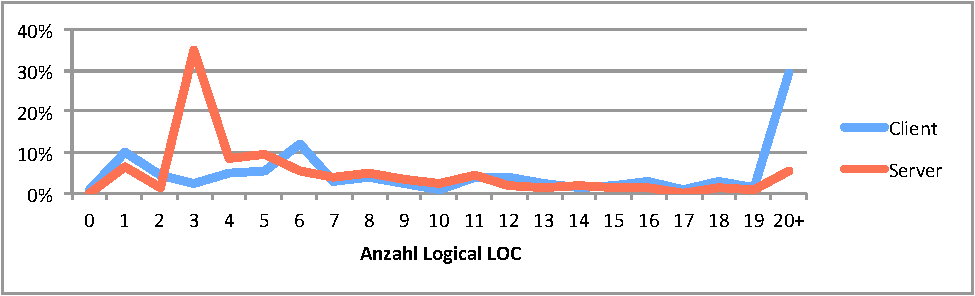
\includegraphics[width=\textwidth]{projectPlan/media/img/methodComplexityLLOC.pdf}
		\centering
		\caption{Anzahl Logical LOC pro Methode}
		\label{fig:methodComplexityLLOC}
	\end{figure}
	In Abbildung\ \ref{fig:methodComplexityParameterCount} ist die Häufigkeit der Anzahl Methoden Parameter aufgezeigt.
	Es ist schön zu erkennen, dass sowohl auf dem Server, wie auch auf dem Client,
	die meisten Methoden keinen oder einen einzigen Parameter besitzen.
	\begin{figure}[H]
		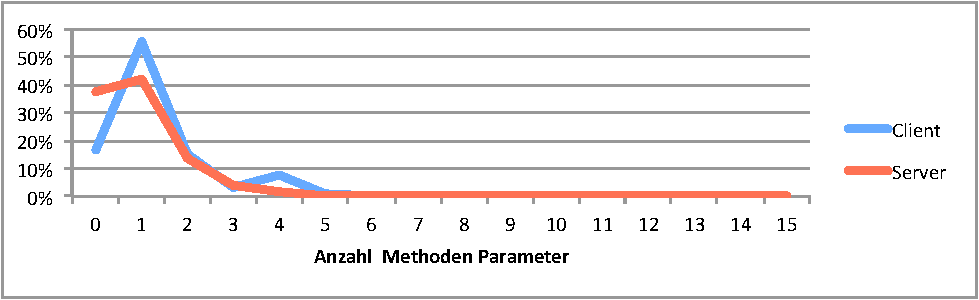
\includegraphics[width=\textwidth]{projectPlan/media/img/methodComplexityParameterCount.pdf}
		\centering
		\caption{Anzahl Parameter pro Methode}
		\label{fig:methodComplexityParameterCount}
	\end{figure}
	Und schliesslich ist die Cyclomatic Complexity in Abbildung\ \ref{fig:methodComplexityCyclomaticComplexity} aufgezeichnet.
	Sie beschreibt, wie viele Operationen eine Methode enthält.
	Beim Server repräsentiert die Spitze am Anfang die Getter und Setter,
	diese sind beim Client so nicht zu sehen,
	da in JavaScript das Konzept von privaten Feldern nicht ausgeprägt eingesetzt wird.
	\begin{figure}[H]
		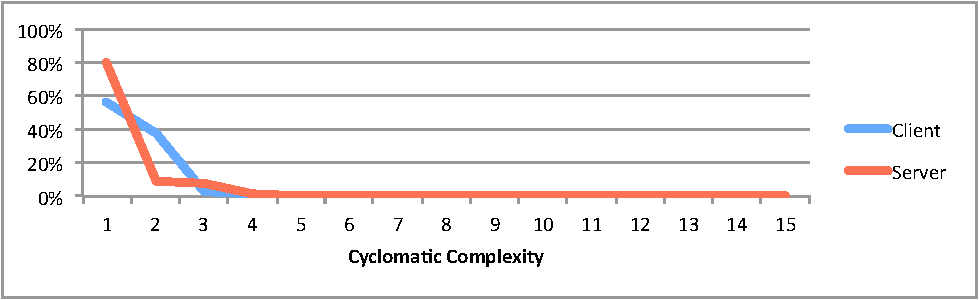
\includegraphics[width=\textwidth]{projectPlan/media/img/methodComplexityCyclomaticComplexity.pdf}
		\centering
		\caption{Cyclomatic Complexity pro Methode}
		\label{fig:methodComplexityCyclomaticComplexity}
	\end{figure}
	
	\subsection{Fazit}
		\eeppi\ hat einen ansehnlichen Umfang und auch eine gute Testabdeckung.
		Ob jetzt jedoch die Codequalität gut ist, lässt sich nur schwer eruieren.
		Ungefähr in der Mitte des Projekts hat ein Mitarbeiter des IFS\footnote{Institut für Software, HSR Hochschule für Technik Rapperswil, \url{http://www.ifs.hsr.ch}} einen Codereview durchgeführt und durchaus positive Bilanz gezogen.
		
		Maurice Halstead hat eine Softwaremetrik entworfen,
		welche die Komplexität der Software berechnet und davon ausgehend einige Kennzahlen liefert.
		Eine davon ist die "'Halstead Bugs"', sie gibt die Fehlerkomplexität an,
		also wie viele Fehler die Software aufgrund der berechneten Komplexität und Grösse statistisch ungefähr enthalten könnte.
		Das heisst aber nicht, dass die Software so viele Fehler enthält,
		sondern die Abstraktion mit Bugs ist nur für das bessere Verständnis der Grössenordnung gedacht.
		\begin{figure}[H]
			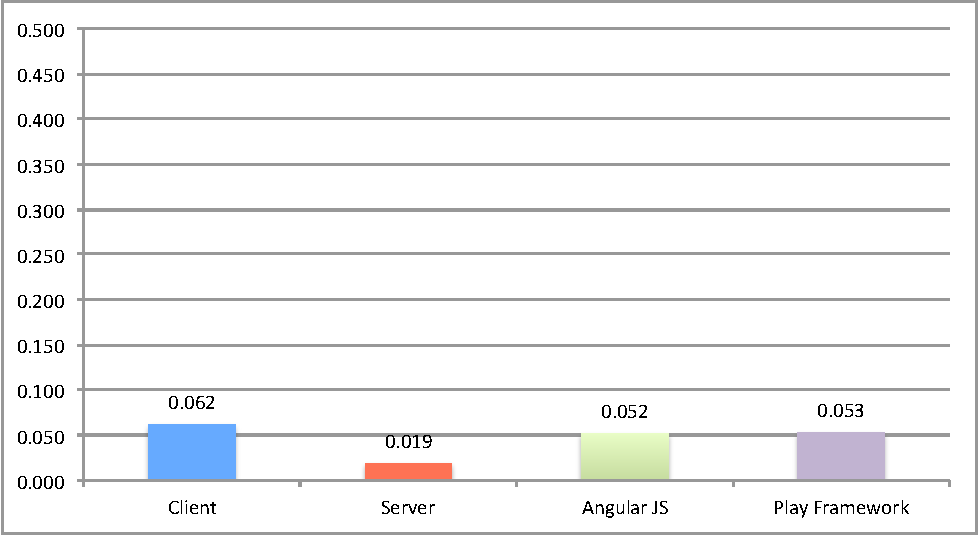
\includegraphics[width=\textwidth]{projectPlan/media/img/halsteadBugsPerMethod.pdf}
			\centering
			\caption{Halstead Bugs pro Methode}
			\label{fig:halsteadBugsPerMethod}
		\end{figure}
		In Abbildung\ \ref{fig:halsteadBugsPerMethod} ist diese Komplexitätsgrösse verglichen mit zwei der durch \eeppi\ eingesetzten Frameworks.
		Der Client weist in etwa die gleiche Komplexität auf,
		wie die beiden Frameworks, der Server eine geringere.
